\documentclass[11pt, a4paper]{article}
\PassOptionsToPackage{hidelinks}{hyperref}
\usepackage[utf8]{inputenc} 
\usepackage{fullpage}
\usepackage{graphicx}
\usepackage{xcolor}
\usepackage{bookmark}
\usepackage{tabularx}
\usepackage{listings}
\usepackage{hyperref}
\usepackage{float}
\usepackage{amsmath}

% Title of your project
\title{Audio Fingerprinting Practical Work}

% Name of deliverable
\newcommand{\deliverableName}{Audio Fingerprinting Practical Work}

% Group names(s)
\author{Javier Novella Ruiz}

% Group number
\newcommand{\groupNumber}{17685207}

% Date for title page, default is today and 
\date{\today}

\makeatletter{}

\setlength{\parindent}{0pt}

\begin{document}

    % Title page based on https://www.latextemplates.com/template/academic-title-page
\begin{titlepage}
  	\newcommand{\HRule}{\rule{\linewidth}{0.3mm}} % Defines a new command for horizontal lines, change thickness here
	\center % Centre everything on the page
	%------------------------------------------------
	%	Headings
	%------------------------------------------------
	
	\textsc{\LARGE Universitat Rovira i Virgili}\\[1.5cm]
	
	\textsc{\Large \deliverableName}\\[0.5cm]
	
	\textsc{\large Multimedia Security}\\[0.5cm]
	
	%------------------------------------------------
	%	Title
	%------------------------------------------------
	
	\HRule\\[0.4cm]
	
	{\huge\bfseries \@title}\\[0.4cm]
	
	\HRule\\[1.5cm]
	
	%------------------------------------------------
	%	Author(s)
	%------------------------------------------------

% 	If you don't want a supervisor, uncomment the two lines below and comment the code above
 %	{\large\textit{Author}}\\
 	{\large\sc\@author} % Your name
	
	%------------------------------------------------
	%	Date
	%------------------------------------------------
	
	\vfill\vfill
		{\large\@date} % Date, change the \today to a set date if you want to be precise
    \vfill\vfill\vfill
	
 %   \footnotesize{Comments: \comments}
%   \vfill\vfill
%    \homepage
%    \vfill
    
    %------------------------------------------------
    % Change log for the plan (can be deleted before delivery)
    % When you update the plan please record what you changed and what the reason for the change. This will be useful for your supervisor.
    %------------------------------------------------
    % \input{./changelog.tex}
	
	%------------------------------------------------
	%	Logo
	%------------------------------------------------
	\vfill
	
\includegraphics[width=0.3\textwidth]{./urvlogo.png}
	\vfill
	 
	
\end{titlepage}


    \tableofcontents

    \newpage

    \section{Introduction}

    The main goal is to implement an audio fingerprinting system that can identify the original track from different audio samples.
    The audio samples are divided in four types: clean samples, filtered samples, noisy samples, noisy filtered samples. These samples
    are short exctracts from the original tracks, adding filters or noise to test the system in harsh conditions.

    \vspace{1em} To the implementation a library of fourty audio files have been used. Each audio file counts with four samples of the previously 
    commented types (clean, filtered, noisy and noisy filtered). This means a total of sixteen samples per original audio file.

    \vspace{1em} The work includes the development of two tools: builddb and identify.
    \begin{list}
        \item builddb: takes the original audios and creates a database with the fingerprint information.
        \item identify: takes a sample and matches the result against the database to return the corresponding original track.
    \end{list}

    \subsection{Technologies used}
    
    After reading the Shazam paper \cite{ShazamAlgorithmPaper} I could imagine an application with a lot of recursivity in the main tasks 
    (reading files, processing files etc.). In programming recursivity usually means computationally demanding, so I tried to avoid slow 
    interpreted languages like Python. The language chosen has been C# \cite{PythonVsCSharp} with the SDK .NET 9.0. The main reason to use this 
    language is that is an object-oriented high-level compiled language. It cheked the application demandings, fast and counts with high-level 
    tools to perform the desired tasks.

    The main packages used for the implementation are:
    \begin{list}
        \item NAudio: library for working with audio files, playback, recording, and processing.
        \item NWaves: digital signal processing (DSP) library for audio analysis.
        \item MessagePack: compact binary serialization format for data exchange.
    \end{list}

    \section{Implementation}

    The implementation is based on the Shazam algorithm \cite{ShazamAlgorithmPaper} and it is divided in two different tools: builddb 
    and identify. Each tool has been developed in a separated C# module \ref{fig:builddb_identify_block_diagram}.

    \begin{figure}[h]
        \centering
        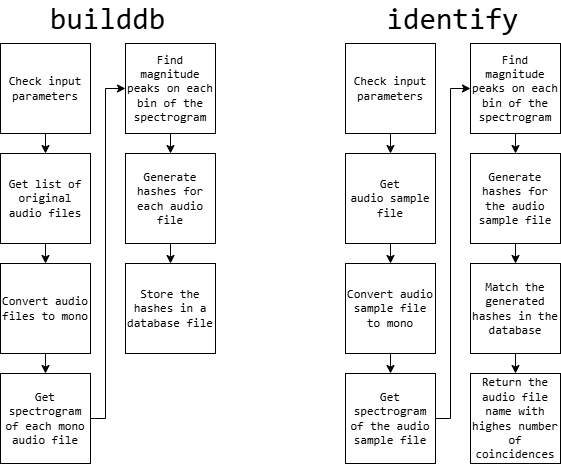
\includegraphics[width=\textwidth]{media/builddb_identify_block_diagram.png}
        \caption{Modules builddb and identify work flow}
        \label{fig:builddb_identify_block_diagram}
    \end{figure}

    The main idea of this process is to split each audio file in small samples and generate a hash for each one. This hash is based on the 
    magnitude peaks as a representative characteristic of the sample. This is done for each audio file and all the hashes are stored in a file 
    that works as a database. During the identification, the same process is carried out with the provided audio sample and then the resultant 
    hashes are collated with the database.

    \subsection{Module builddb}

    The module builddb 

    \begin{list}

    \end{list}



    \newpage

    \begin{thebibliography}{11}

    \bibitem{ShazamAlgorithmPaper}
    A. L.-C. Wang, \textit{An Industrial-Strength Audio Search Algorithm}.  
    Shazam Entertainment, Ltd.  
    Available at \url{https://www.ee.columbia.edu/~dpwe/papers/Wang03-shazam.pdf}.

    \bibitem{PythonVsCSharp}
    TCM Security, \textit{Python vs C#: Which One is Better in 2023?}.  
    Available at \url{https://tcm-sec.com/python-vs-c-sharp/#:~:text=Performance%20and%20Speed,only%202%20seconds%20to%20run}.

    \end{thebibliography}

\end{document}
